\section{Discussion} \label{sec:discussion}

\subsection{Limitations \& Known Issues} \label{sec:discussion:limitations}

The ISR pipeline developed for LSSTCam removes the dominant instrumental signatures, but several effects remain partially corrected, unmodeled, or unmasked.
The paragraphs below summarize known limitations (instrumental systematics not fully corrected, edge cases, validity constraints, etc.) for interpreting DP2 data, our recommendations for handling them in the context of DP2 science, and plans for near-term improvements expected before Data Release~1 (DR1).

\paragraph{Flares}
Some science images contain localized, bright flare-like structures.\todo{Quantify?}
They appear as elongated trails that begin at a detector edge and fade with a wavelength-dependent power-law profile consistent with attenuation of light in silicon at that wavelength.
The light is likely scattered from bright stars: focused starlight may reflect from the beveled edge of the silicon mount and enter a neighboring detector through its side, although this mechanism is not yet confirmed.
Similar structures appear in some flat-field images as many small edge flares (referred to as a ``comb'' pattern), possibly linked to the rough-cut silicon edge.
So far, these features have been seen only in $y$-band, with both focused and unfocused illumination, and they are transient, consistent with a dependence on the chance alignment of bright stars with the focal-plane array.
They are not yet fully characterized or masked in DP2 processing.
Science users should treat anomalously bright detections/extended objects near detector edges with caution in $y$-band single-visit and difference images, and verify suspect sources by visual inspection.

\paragraph{Residual non-linearity wiggles}
The double-spline non-linearity model (\S\ref{sec:calibration-production:linearity}) removes the dominant signal-dependent departure from linear response, but small quasi-oscillatory residuals remain as a function of signal level.
They appear as low-amplitude, signal-dependent structure in linearized images.
These ``wiggles'' are irregular, clearly observed beyond noise fluctuations, and they do not correlate with measured properties of the input flat-field images (e.g. time, temperature) or with channel on a detector or across the focal plane.
These residuals are well below current science requirements and are left uncorrected in DP2, but further characterization is in progress.\todo{Quantify?}

\paragraph{Differential non-linearity (DNL)}
The DP2 linearizer corrects average amplifier non-linearity but does not yet apply a full low-signal differential non-linearity correction.
This limitation reflects the difficulty of delivering flat-field illumination below 100 ADU/pixel with the in-dome calibration system.
Users should exercise caution when relying on photometric or astrometric measurements at low signal levels, in particular when relying on $u$-band sky-background estimates from later processing steps, where backgrounds are typically at or below 100 ADU/pixel.
Count dithering in ISR (\S\ref{sec:isr-science}) provides interim mitigation until a dedicated DNL correction is measured and deployed.

\paragraph{Detector vignetting models}
Flat-field calibrations measure relative pixel and filter quantum efficiencies and throughputs under uniform illumination, but they require an accurate model of optical vignetting across the focal plane.
Improved vignetting models, informed by larger calibration datasets and cross-checks against on-sky stellar photometry, are planned for future calibration epochs to reduce focal-plane non-uniformity.\todo{Quantify?}

\paragraph{Color-dependent BFE corrections}
The BFE is color dependent because its amplitude depends on photon conversion depth in silicon and on the path length over which the transverse electric field acts on drifting electrons.
Laboratory and commissioning measurements show that the effect is chromatic \citep[$a_{00}^{y-band} = 0.94 \times a_{00}^{r-band}$, see][]{2024PASP..136d5003B}.
The electrostatic BFE model used in DP2 (\S\ref{sec:calibration-production:bf}) is fit from PTC covariances and applies a single wavelength-averaged correction per detector, derived in the band of the PTC input flats.
Because the effect is strongest near the bottom of the potential well and the front of the chip, calibrations for $u$ through $i$ bands are approximately consistent as most light in those bands converts to photoelectrons within the first few microns.
Separate calibrations are appropriate for $z$- and $y$-band light, which typically  convert far deeper into the silicon.
Boundary-shift calibrations can be color-corrected by assuming a flat incident spectral energy distribution in each filter band and a depth-conversion model in silicon.
These corrections were not enabled in DP2 because validation was incomplete, but they are expected for DR1.
Until then, PSF photometry and shape measurements of bright sources, especially in redder bands, may retain small flux- and filter-dependent biases.\todo{Quantify?}

\paragraph{Fringing}
Fringing is an interference pattern produced when narrow-band emission reflects within the thin, back-illuminated silicon of LSSTCam CCDs.
It is driven primarily by night-sky emission lines and becomes appreciable in the $z$- and $y$-bands, where the silicon is increasingly transmissive and OH and other atmospheric lines contribute strongly to the background.
In-dome flat-field exposures (\S\ref{sec:calibration-production:flats}) imprint and partially divide out a fringe pattern, but the fringing amplitude and phase in science images depend on the time-varying on-sky spectrum and therefore are not fully canceled by flat-fielding alone.
The DP2 ISR pipeline (\S\ref{sec:isr-science}) does not include a dedicated fringe-subtraction step.
Residual fringe structure is visible at low surface brightness in $z$- and $y$-band visit images and can bias wide-aperture photometry.\todo{Quantify?}
Fringing models developed by \citet{2023PASP..135c4503G} and corresponding corrections are under development and expected for DR1; until then, users analyzing faint extended emission or precision surface-brightness measurements in redder bands should inspect visit images for quasi-periodic fringe patterns and treat affected regions with appropriate caution.

\paragraph{Masking}
Several limitations for the defects exist for DP2:
\begin{itemize}
\item vampire pixels
\item edge bleeds
\end{itemize}\todo{Quantify?}
Further developments will provide better support and masking for LSST data releases.

\subsection{Calibration Sensitivity to Camera Sequencer} \label{sec:discussion:sequencer}
Because many instrument signatures depend on the electronic configuration of the sensor and the timing of the readout, therefore a change to the sequencer can invalidate calibration products built under the previous one.
\citet{2026arXiv260631806M} describe how the LSSTCam sequencer has evolved since the camera arrived at the summit.
The most significant on-sky change was the move to a more relaxed total focal plane readout time from 2\,s to 3\,s.
The extra time was spent on a longer per-row readout interval, while the other sequencer parameters tuned during laboratory testing were left unchanged.
This lowered the read noise of the E2V sensors by about 0.5\,e$^-$, while the ITL sensors were largely unaffected \citep{2026arXiv260631806M}.

DP2 includes science data taken under two sequencers: the original 2\,s \texttt{2s\_v30} sequencer (epoch~1) and the \texttt{3s\_v1} sequencer (epochs~2 and 3; Figure~\ref{fig:calibepoch}).
Each sequencer required its own set of calibrations.
The move to 3\,s readout changed the read noise and bias structure measured in the overscan, and it also changed the size of the crosstalk signal, so the crosstalk coefficients had to be measured again (\S\ref{sec:calibration-production:xtalk}).
A further update, \texttt{3s\_v2}, was introduced after the DP2 data cutoff on January 6, 2026.\todo{Briefly state what changed between \texttt{3s\_v1} and \texttt{3s\_v2}.}
Throughout DP2, detector~101 (R23\_S02) showed signal-dependent correlated noise.
This noise interfered with the photon transfer curve calibration (\S\ref{sec:calibration-production:ptc}) and with the measurement of both gain and read noise for that detector.
The correlated noise disappeared with the move to the \texttt{3s\_v2} sequencer.
No \texttt{3s\_v2} data or calibrations are included in the DP2 release, but \texttt{3s\_v2} is the sequencer used for survey operations from now on.
For that reason, the calibration products shown in this paper are the \texttt{3s\_v2} products.
The algorithms are the same for all sequencers; only the input exposures and the resulting calibration products differ in.

\begin{figure*}[t]
    \centering
    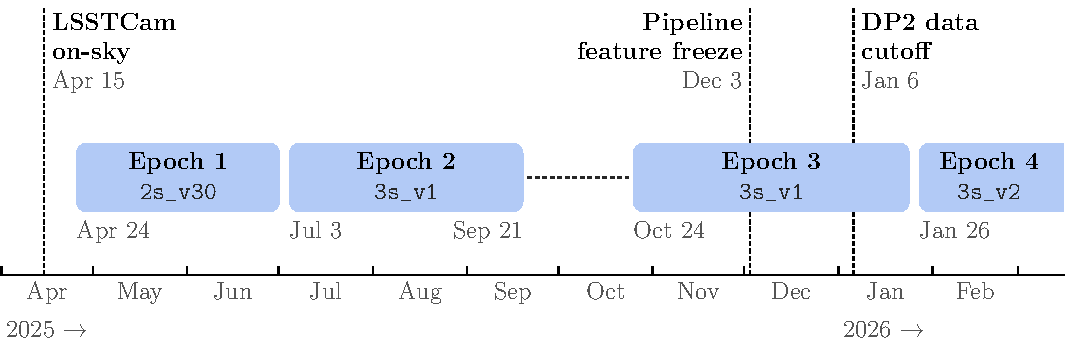
\includegraphics[width=0.75\textwidth]{figures/calibration-epochs-timeline.pdf}
    \caption{Timeline of the observing periods and calibration epochs for LSSTCam during commissioning and pre-survey operations included in DP2.
    The timeline begins with LSSTCam going on-sky on 2025 April 15; the first science data included in DP2 was taken on 2025 April 24.
    DP2 science data are separated into calibration epochs, which are set by changes to the CCD operating mode (sequencer) or by power cycles for maintenance.
    Blue boxes mark the interval covered by each calibration epoch and are labeled with the sequencer in use: epoch~1 (from 2025 April 24, \texttt{2s\_v30}), epoch~2 (2025 July 3 to September 21, \texttt{3s\_v1}), and epoch~3 (from 2025 October 24, \texttt{3s\_v1}).
    Epoch~4 (from 2026 January 26, \texttt{3s\_v2}) follows the DP2 data cutoff on 2026 January 6.
    The calibrations shown in this paper are the most recent (\texttt{3s\_v2}) set, even though no data from this epoch were released in DP2.
    The dotted segment marks an engineering and maintenance downtime between 2025 September 21 and October 24 that is not covered by a calibration epoch.
    The feature freeze for v30 of the LSST Data Management (DM) Science Pipelines software was 2025 December 3.}
    \label{fig:calibepoch}
\end{figure*}